\documentclass[a4paper,10pt]{beamer}
\usepackage[utf8]{inputenc}
\usepackage{color}
\usepackage{colortbl}
\usepackage{xcolor}
\usepackage{caption}
\usepackage{ragged2e}
\usepackage{hyperref}
\usepackage{marvosym}
\renewcommand{\figurename}{Figura}
\usetheme{Warsaw}

%Enumerar figuras
\setbeamertemplate{caption}[numbered]


\logo{
\includegraphics[scale=0.05]{logoUNAM}}
\begin{document}

\begin{frame}
\Large
\title{Tubos fotomultiplicadores y fotodiodos}
\author{Favio Vázquez}
\date{$1^{ro}$ de septiembre de 2015}

Láminas disponibles en \href{https://github.com/FavioVazquez/DeteccionRayosCosmicos-PCF}{(\color{blue} GitHub})

\maketitle
\end{frame}

\section[\'Indice]{}
\frame{

\Large{\'Indice}

\tableofcontents

}

\section{Introducción}
\begin{frame}[allowframebreaks]{Introducción}
\begin{justify}
 El uso masivo de la cuenta de centelladores en la detección y espectroscopia sería 
 imposible sin la disponibilidad de dispositivos que nos permitiera convertir la 
 salida de luz débil de un pulso de centellador, en una señal eléctrica medible. 
 
 \vspace{.3cm}
 
 Los tubos fotomultiplicadores (FM) cumplen con esta tarea muy bien, convirtiendo señales 
 de luz que constan típicamente de no más que unos cientos de fotones, en un pulso 
 de corriente utilizable sin añadir una gran cantidad de ruido aleatorio a la señal.
 
\framebreak

 Existe una gran variedad comercial de estos tubos sensibles a diversas longitudes de onda,
 ultravioleta, luz visible, cercana a la infrarroja y otras del espectro electromagnético.
 
 \vspace{.3cm}
 
 \textbf{Usos}:
 
 \begin{center}
   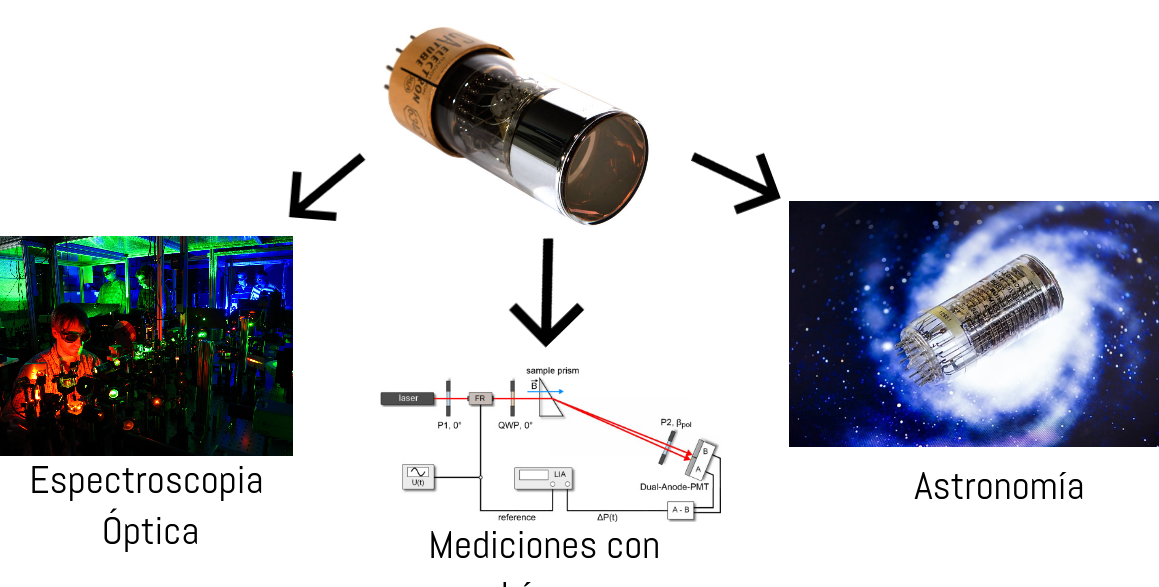
\includegraphics[scale=0.2]{fig1}
 \end{center}

 
 \end{justify}
\end{frame}

\section{Estructura simplificada de un Tubo FM}
\begin{frame}[allowframebreaks]{Estructura simplificada de un Tubo FM}
 
 \begin{columns}[c]
  \column{1.5in}
  \begin{figure}
  \center
   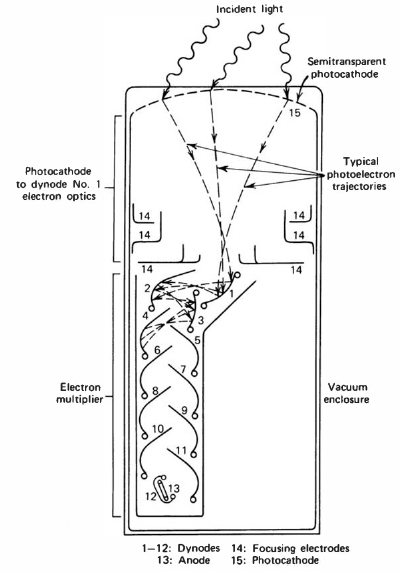
\includegraphics[scale=0.28]{fig2}
   \caption{Elementos básicos de un tubo FM}
  \end{figure}

  \column{2.5in}
  \begin{justify}
   
   \footnotesize{Una envoltura (usualmente de vidrio) sirve como una barrera de presión
   para mantener las condiciones de vacío dentro del tubo, que son requeridas
   para que los electrones de bajas energías puedan ser acelerados eficientemente
   por los campos eléctricos internos.
   
   \vspace{.3cm}
   
   Los dos mayores componentes dentro del tubo son una capa fotosensible, llamada
   el \emph{fotocátodo}, acoplado a una \emph{estructura multiplicadora de fotones}.
   El fotocátodo sirve para convertir la mayor cantidad posible de fotones de luz
   en electrones de baja energía.
   
   \vspace{.3cm}
   
   La sección de multiplicadora de electrones en un tubo FM provee una geometría
   de colección eficiente para los fotoelectrones, y sirve como un amplificador
   casi ideal para incrementar en altas cantidades su número.}
   
   
  \end{justify}

 \end{columns} 
 
 \framebreak
 
  \begin{figure}
  \center
   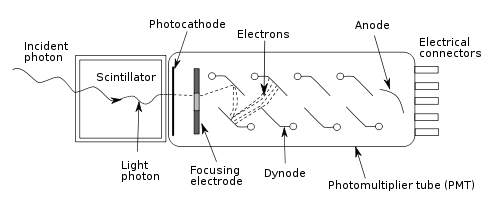
\includegraphics[scale=0.4]{fig3}
   \caption{Elementos básicos de un tubo FM}
  \end{figure}
  
  \begin{justify}
   \footnotesize{
   Luego de una amplificación a través de la estructura multiplicadora, un pulso 
   típico de centellador dará lugar a unos $10^7-10^10$ electrones, suficientes
   para servir de señal de carga para el evento original de centelleo. Esta carga
   es colectada convencionalmente en el ánodo o la etapa de salida de la estructura
   multiplicadora.
   
   \vspace{.3cm}
   
   Tubos típicos, cuando son iluminados por un pulso de luz de muy corta duración,
   producirán un pulso de electrones en un tiempo aproximado de unos pocos nanosegundos
   luego de un tiempo de espera de $20-50$ ns.}
   \end{justify}
    
\end{frame}

\section{El fotocátodo}

\begin{frame}
\begin{center}
 \Huge{\color{blue}El fotocátodo} \\
 \vspace{1cm}
 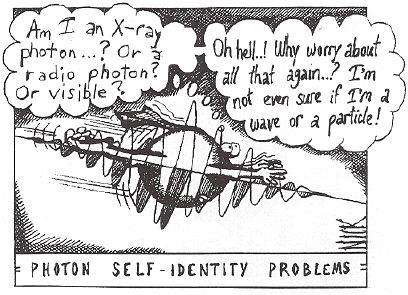
\includegraphics[scale=0.7]{fig4}
\end{center}
\end{frame}


\subsection{El proceso de fotoemisión}
\begin{frame}{El proceso de fotoemisión}
 
 \begin{justify}
  El primer paso realizado por el tubo FM es la conversión de fotones de luz incidente
  en electrones. Este proceso de foto emisión puede pensarse que ocurre en tres etapas
  secuenciales:
  
   \begin{enumerate} [<+->]
  \item La absorción de un fotón incidente y transferencia de energía a un electrón
  dentro del material fotoemisivo,
  \item la migración de ese electrón a la superficie y,
  \item el escape del electrón de la superficie del fotocátodo. 
  \begin{block}{Notas importantes}
  \footnotesize{\begin{justify}La energía que puede transferirse del fotón al electrón en el primer paso está
  dada por la energía cuántica del fotón $hv$ (típicamente $\sim 3$ eV). En el paso 2, alguna de esa energía
  se perderá por las colisiones de electrón-electrón. En el paso 3, debe haber
  la suficiente energía restante para que el electrón pase el potencial barrera
  inherente (\emph{función de trabajo.} (comúnmente $> 3$ o $4$ eV, pero para 
  metales $\sim 1.5-2$ eV)\end{justify}}
 \end{block}
 \end{enumerate}
 
 \end{justify}
  
\end{frame}

\subsection{Emisión espontánea de electrones}
\begin{frame}{Emisión espontánea de electrones}
 \begin{justify}
 La barrera de potencial superficial influencia una propiedad importante de los
 fotocátodos: \emph{el ruido termiónico}. La conducción normal de electrones
 adentro del material del fotocátodo siempre tendrá algo de energía cinética térmica
 que, a temperatura ambiente, se aproximará a los $0.025$ eV. 
 
 \vspace{.3cm}
 
 Si ese electrón está cerca de la superficie, puede escapar y dar lugar a una señal
 inducida térmica espontánea.
  
\begin{block}{Nota relevante}
 \begin{justify}
  En los metales, la tasa de emisión térmica es baja $(\sim 100 \text{m}^2\cdot \text{s})$
  debido a su potencial de barrera relativamente alto. En los semiconductores, el bajo 
  potencial de barrea lleva a tasas de emisión térmicas tan altas como $10^6-10^8 \text{m}^2\cdot \text{s}$
 \end{justify}
 \end{block}
\end{justify}
\end{frame}

\subsection{Fabricación de fotocátodos}
\begin{frame}{Fabricación de fotocátodos}
 \begin{justify}
  
  \small{Los fotocátodos pueden ser construidos tanto por capas opacas o semitransparentes.
  Un fotocátodo opaco es fabricado normalmente con un grosor un poco más grande 
  que la profundidad de escape máxima\footnotemark y es soportado por un material
  de respaldo grueso. Los fotocátodos semitransparentes generalmente no son más 
  gruesos que la profundidad de escape, son depositados en un respaldo transparente 
  (usualmente el final del vidrio del tubo FM).}
  
  \begin{block}{Nota relevante}
  \begin{justify}
   Debido a que son más fácilmente adaptables a diseños de tubo que usan una 
   ventana final plana, los fotocátodos semitransparentes son más comunes en los
   tubos FM diseñados para conteo de centelladores.
   \end{justify}
  \end{block}
  
  \begin{exampleblock}{Nota experimental}
  \begin{justify}
   Las variaciones en el espesor darán lugar a cambios correspondientes en la sensitividad 
   del fotocátodo y pueden ser una fuente de pérdida de resolución en los conteos de 
   centelladores (el problema es $\propto$ al diámetro del tubo).
   \end{justify}
  \end{exampleblock}

  \footnotetext[1]{Profundidad máxima del material, en la que los electrones puedan
  alcanzar la superficie y superar el potencial de barrera.}
  
 \end{justify}

\end{frame}

\subsection{Eficiencia cuántica y respuesta espectral}
\begin{frame}[allowframebreaks]{Eficiencia cuántica y respuesta espectral}
 \begin{justify}
  
  \small{La sensitividad de los fotocátodos se mide comúnmente en el ámbito
  de la física, y con gran significación para el conteo de centelladores
  en términos de la \emph{eficiencia cuántica (EC)} del fotocátodo.
  La eficiencia cuántica se define simplemente como}
  
  \begin{equation}
   EQ = \frac{\text{número de fotoelectrones emitidos}}{\text{número de fotones incidentes}}
  \end{equation}

  \vspace{.2cm}
  
  \small{La eficiencia cuántica sería de $100\%$ para un fotocátodo ideal. Pero
  debido a las limitaciones que les he mencionado, los fotocátodos
  comunes tienen una eficiencia cuántica máxima de $20-30\%$.}
  
  \begin{columns}[c]
    \column{2in}
  \begin{block}{Nota relevante}
  \begin{justify}
   La eficiencia cuántica de cualquier fotocátodo será fuertemente una 
   función de la longitud de onda o la energía cuántica de la luz incidente.
   \end{justify}
  \end{block}
    \column{2in}
  \begin{exampleblock}{Nota experimental}
  \begin{justify}
  Una consideración para seleccionar un fotocátodo es buscar una alta
  eficiencia cuántica sobre el rango de longitudes de onda en el 
  cual el espectro de emisión del centellador es concentrado.
   \end{justify}
  \end{exampleblock}
  \end{columns}

  \pause
  
  \begin{columns}[c]
  \column{2in}
  \begin{figure}
   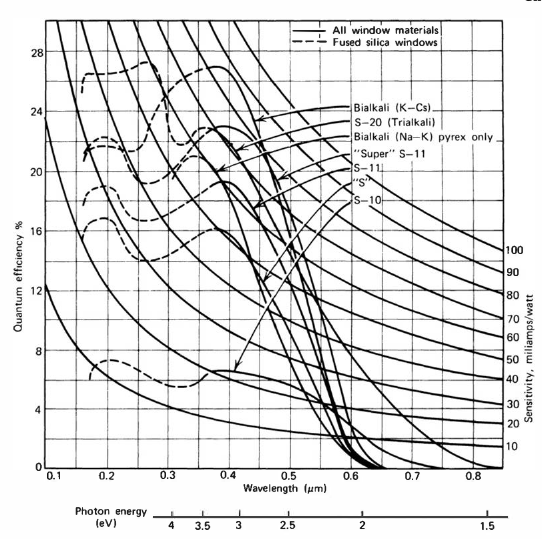
\includegraphics[scale=0.28]{fig5}
   \caption{La eficiencia cuántica es función de la longitud de onda
   o de la energía cuántica de la luz incidente}
  \end{figure}
  
  \column{2in}
  \begin{justify}
  \footnotesize{A una $\lambda$ lo suficientemente alta el electrón no tiene la suficiente
  energía para escapar la superficie del fotocátodo y la respuesta se 
  hace cero. Para vidrio normal, el límite será a $\lambda \sim 350$ nm,
  que es usualmente adecuado para la mayoría de los materiales de centelladores.}
  \end{justify}
  
  \begin{exampleblock}{Nota experimental}
   \begin{justify}
   \footnotesize{Una medida alternativa para la EQ es usada en el conteo de 
   centelladores. Debido al uso extendido de yoduro de sodio 
   activado con talio como cristal de centelleo, se habla de EQ 
   en términos de el número de fotoelectrones producidos por un
   fotocátodo dado por keV de pérdida de energía en un cristal
   de NaI(Tl) para el cual casi toda la luz es colectada.}
   \end{justify}
  \end{exampleblock}

  \end{columns}

  \pause
  
  \textbf{Materiales actuales para la construcción de fotocátodos}:
  
  \begin{itemize}
   \item \begin{justify}Materiales multialcalinos basados en el compuesto Na$_2$KSb,
   preparados por activación con una pequeña cantidad de cesio 
   $\Rightarrow$ EQ $\sim 30\%$.\end{justify}
   \item \begin{justify}Materiales bialcalinos basados en K$_2$CsSb activados con
   oxígeno y cesio $\Rightarrow$ $45\%$ a los 350 nm de máxima respuesta.\end{justify}
   \item \begin{justify}Materiales ultrapuros que reducen las trampas de electrones,
   reduciendo reflexiones desde el fotocátodo mediante una introducción
   de de una capa antireflejante entre él y la envoltura de vidrio.\end{justify}
   \item \begin{justify}Estructuras prismáticas con un alto radio de superficie 
   a volumen para aumentar la probabilidad de escape de fotoelectrones.\end{justify}
  \end{itemize}

  
 \end{justify}
\end{frame}



\end{document}
